\documentclass[12pt,a4paper]{article}

\usepackage[T1]{fontenc}
\usepackage[utf8]{inputenc}
\usepackage[brazil]{babel}
\usepackage{amsmath, amssymb, amsfonts, amsthm}
\usepackage{booktabs}
\usepackage[left=3cm, top=3cm, right=2cm, bottom=2cm]{geometry}
\usepackage{siunitx}
\usepackage{graphicx} % Required for inserting images
\usepackage{indentfirst}
\usepackage{multicol}
\usepackage{float}
\usepackage{caption}
\usepackage{cancel}


\sisetup{output-decimal-marker={,}}

\title{An\'alise da Energia de Liga\c{c}\~ao Nuclear e da Energia de Liga\c{c}\~ao por N\'ucleon}
\author{Jefferson Vasconcelos teles de Almeida}
\date{\today}

\begin{document}

\maketitle

\begin{abstract}
Este artigo apresenta uma discuss\~ao dos resultados obtidos por um script em Python para c\'alculo da energia de liga\c{c}\~ao total do n\'ucleo ($E_B$) e da energia de liga\c{c}\~ao por n\'ucleon ($E_B/A$). A an\'alise foi feita para diferentes is\'otopos est\'aveis, cobrindo n\'ucleos leves, m\'edios e pesados. Os resultados reproduzem o comportamento esperado da curva de energia de liga\c{c}\~ao por n\'ucleon: crescimento nos n\'ucleos leves, m\'aximo na regi\~ao do ferro e queda gradual para n\'ucleos muito pesados.
\end{abstract}

\section{Introdu\c{c}\~ao}
A estabilidade nuclear est\'a diretamente relacionada \`a energia de liga\c{c}\~ao. Essa grandeza representa a energia necess\'aria para separar um n\'ucleo em seus pr\'otons e n\'eutrons. Quanto maior a energia de liga\c{c}\~ao por n\'ucleon, mais est\'avel tende a ser o n\'ucleo.

Neste trabalho, foram utilizados dados de massa at\^omica experimental para calcular:
\begin{itemize}
	\item a energia de liga\c{c}\~ao total $E_B$;
	\item a energia de liga\c{c}\~ao por n\'ucleon, definida por:
\end{itemize}

\begin{equation}
\frac{E_B}{A},
\end{equation}

em que $A$ \`e o n\'umero de massa do n\'ucleo.

\section{Metodologia}
O script calcula inicialmente o n\'umero de n\'eutrons por:
\begin{equation}
N = A - Z,
\end{equation}
onde $Z$ \`e o n\'umero de pr\'otons.

A energia de liga\c{c}\~ao total \`e obtida por:
\begin{equation}
E_B = \left[ Zm_H + Nm_n - m_{\text{at\^omica}} \right] c^2,
\end{equation}
com $m_H$ a massa do \`atomo de hidrog\^enio, $m_n$ a massa do n\^eutron e $c^2 = \SI{931.5}{MeV/u}$.

Em seguida, calcula-se:
\begin{equation}
\frac{E_B}{A} = \text{energia de liga\c{c}\~ao por n\'ucleon}.
\end{equation}

Por fim, os valores foram ordenados em $A$ crescente e representados em gr\'afico de $E_B/A$ versus $A$.

\section{Resultados}
A Tabela~\ref{tab:resumo} apresenta um recorte dos resultados obtidos pelo script.

\begin{table}[h]
\centering
\caption{Exemplos de energia de liga\c{c}\~ao total e por n\'ucleon.}
\label{tab:resumo}
\begin{tabular}{lccc}
\toprule
Is\'otopo & $A$ & $E_B$ (MeV) & $E_B/A$ (MeV/n\'ucleon) \\
\midrule
B-11   & 11  & 76,21   & 6,928 \\
C-12   & 12  & 92,16   & 7,680 \\
O-16   & 16  & 127,62  & 7,976 \\
Ca-40  & 40  & 342,06  & 8,552 \\
Fe-56  & 56  & 492,26  & 8,790 \\
Pb-208 & 208 & 1636,45 & 7,868 \\
U-238  & 238 & 1801,71 & 7,570 \\
Pu-244 & 244 & 1836,08 & 7,525 \\
\bottomrule
\end{tabular}
\end{table}

\begin{figure}[h]
    \centering
    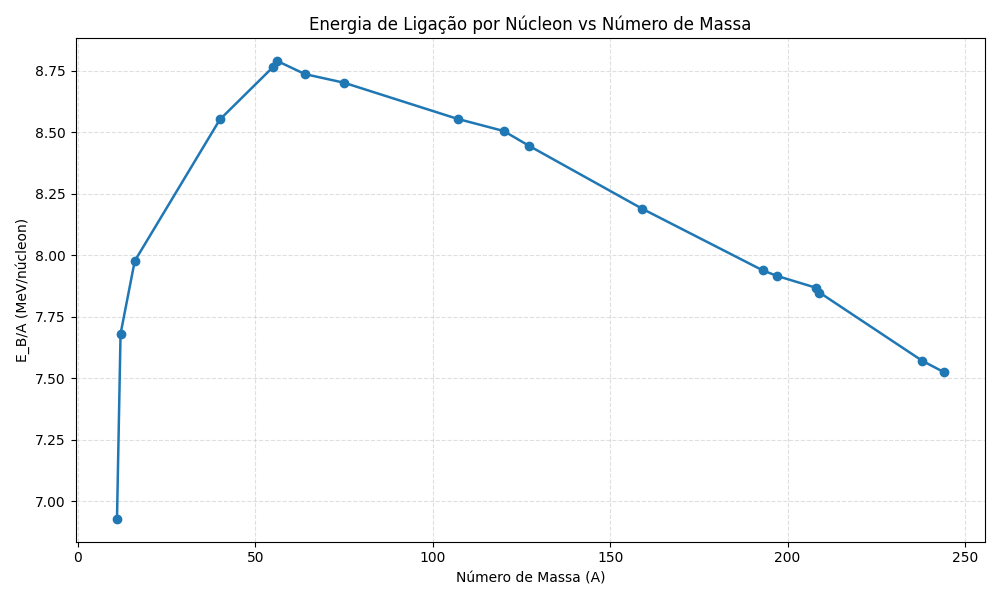
\includegraphics[width=0.9\linewidth]{Figure_1.png}
	\caption{Energia de liga\c{c}\~ao por n\'ucleon em fun\c{c}\~ao do n\'umero de massa.}
    \label{fig:placeholder}
\end{figure}




\section{Discuss\~ao}
Os resultados mostram tr\^es regi\~oes principais:
\begin{enumerate}
	\item \textbf{N\'ucleos leves:} o valor de $E_B/A$ cresce rapidamente com $A$. Isso indica que adicionar n\'ucleons aumenta significativamente a estabilidade nesse intervalo.
	\item \textbf{Regi\~ao intermedi\'aria (pr\'oxima do ferro):} observa-se um m\'aximo em torno de Fe-56, com $E_B/A \approx \SI{8.79}{MeV/nucleon}$. Essa regi\~ao corresponde aos n\'ucleos mais est\'aveis.
	\item \textbf{N\'ucleos pesados:} para $A$ maiores, $E_B/A$ decresce de forma gradual. Isso ocorre devido ao aumento do efeito repulsivo coulombiano entre os pr\'otons, reduzindo a liga\c{c}\~ao m\'edia por n\'ucleon.
\end{enumerate}

Essa estrutura da curva explica dois processos fundamentais em f\'isica nuclear:
\begin{itemize}
	\item \textbf{Fus\~ao} de n\'ucleos leves libera energia, pois leva o sistema para valores maiores de $E_B/A$.
	\item \textbf{Fiss\~ao} de n\'ucleos muito pesados tamb\'em libera energia, pois os produtos tendem a ter $E_B/A$ mais alto que o n\'ucleo inicial.
\end{itemize}

\section{Conclus\~ao}
O script implementado permitiu calcular corretamente a energia de liga\c{c}\~ao total e a energia de liga\c{c}\~ao por n\'ucleon para uma s\'erie de is\'otopos. A tend\^encia observada no gr\'afico de $E_B/A$ em fun\c{c}\~ao de $A$ est\'a de acordo com a teoria: aumento nos n\'ucleos leves, m\'aximo na regi\~ao do ferro e queda para n\'ucleos pesados.

Assim, os resultados num\'ericos e gr\'aficos confirmam a interpreta\c{c}\~ao f\'isica da estabilidade nuclear e sua rela\c{c}\~ao com os mecanismos de fus\~ao e fiss\~ao.

\end{document}
